% === [ Appendix ] =============================================================

\onecolumn

\appendix
\setcounter{secnumdepth}{0}
\section{Appendices}
\setcounter{secnumdepth}{3}
\renewcommand{\thesubsection}{\Alph{subsection}}

% --- [ Local variable example ] -----------------------------------------------

\subsection{Local variable example}
\label{app:local_variable_example}

\begin{figure}[htbp]
	\centering
	\begin{subfigure}[ht]{0.3\textwidth}
		\centering
		\lstinputlisting[language=c, style=go, breaklines=false]{inc/printf.c}
		\caption{Example C source code.}
		\label{fig:local_variable_example_c}
	\end{subfigure}
	\qquad
	\begin{subfigure}[ht]{0.65\textwidth}
		\centering
		\lstinputlisting[language=nasm, style=nasm, breaklines=false]{inc/printf.asm}
		\caption{Corresponding assembly code in NASM syntax.}
		\label{fig:local_variable_example_asm}
	\end{subfigure}
	\caption{Local variable example used to illustrate different aspects of variable recovery and type analysis.}
	\label{fig:local_variable_example}
\end{figure}

% --- [ Structure type example ] -----------------------------------------------

\clearpage

\subsection{Structure type example}
\label{app:struct_example}

\begin{figure}[htbp]
	\centering
	\begin{subfigure}[ht]{0.3\textwidth}
		\centering
		\lstinputlisting[language=c, style=go, breaklines=false]{inc/struct.c}
		\caption{Struct example C source code.}
		\label{fig:struct_example_c}
	\end{subfigure}
	\qquad
	\begin{subfigure}[ht]{0.65\textwidth}
		\centering
		\lstinputlisting[language=nasm, style=nasm, breaklines=false]{inc/struct.asm}
		\caption{Corresponding assembly code in NASM syntax.}
		\label{fig:struct_example_asm}
	\end{subfigure}
	\caption{Struct example used to illustrate type recover of structure types.}
	\label{fig:struct_example}
\end{figure}

% --- [ Structure pointers with offsets ] --------------------------------------

\clearpage

\subsection{Structure pointers with offsets}
\label{app:structure_pointers_with_offsets}

When decompiling the assembly of the structure type example (see figure \ref{fig:struct_example_asm}) using the state-of-the-art decompiler IDA Hex-Rays (version 7.1.180227), an issue in the type recovery of pointers to structure types has been identified; where IDA lacks a type representation of \textit{pointing into a structure type at an offset}.

The type of \texttt{p} in figure \ref{fig:ida_struct} should be \textit{pointer to T at offset 5}, but C lacks a representation for such a type, and IDA seem to lose this information in its internal representation; thus resulting in suboptimal type recovery, as the structure field accesses \texttt{p->y}, \texttt{p->x} and \texttt{p->name} are not recovered at line 13, 14 and 15, respectively.

\begin{figure}[htbp]
	\centering
	\begin{subfigure}[ht]{0.45\textwidth}
		\centering
		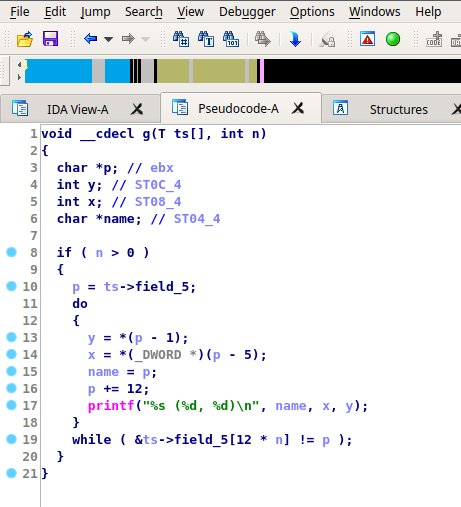
\includegraphics[width=\textwidth]{inc/ida_struct_1.png}
		\caption{Pointer to char; correct representation but loses information about \texttt{T}.}
		\label{fig:ida_struct_1}
	\end{subfigure}
	\qquad
	\begin{subfigure}[ht]{0.45\textwidth}
		\centering
		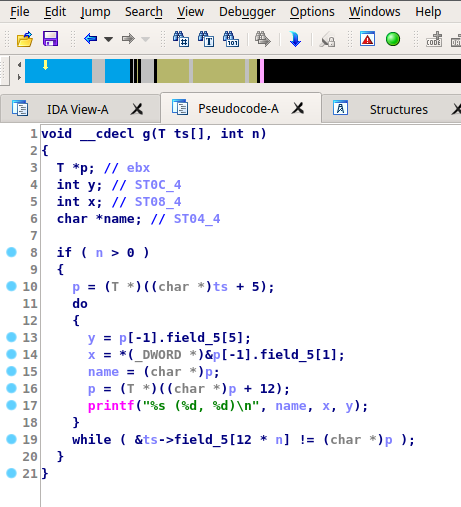
\includegraphics[width=\textwidth]{inc/ida_struct_2.png}
		\caption{Pointer to \texttt{T}; incorrect representation.}
		\label{fig:ida_struct_2}
	\end{subfigure}
	\caption{IDA fails to recover (or has no valid internal representation of) the pointer type of \texttt{p}, which should be \textit{pointer to T at offset 5}.}
	\label{fig:ida_struct}
\end{figure}
